\section{Spatiotemporal Extent}
\label{sec:Spatiotemporal}
%%%%%%%%%%%%%%%%%%%%%%%%%%%%%%%%%%%%%%%%%%%%%%%%%%%%%%%%
\begin{figure}[h!]
\begin{center}
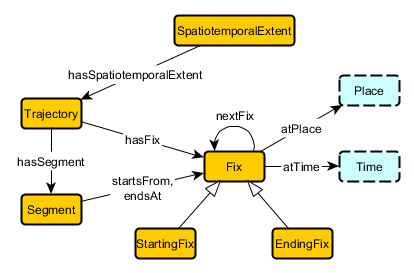
\includegraphics[width=.8\textwidth]{figures/ste}
\end{center}
\caption{Schema Diagram for the Spatiotemporal Extent Pattern. The visual notation is explained in Chapter \ref{chap:prelims}.}
\label{fig:Spatiotemporal}
\end{figure}
\subsection{Summary}
\label{sum:Spatiotemporal}
%%%%%%%%%%%%%%%%%%%%%%%%%%%%
This pattern is adapted from \cite{ste}.

The rest of the axioms can be found in Section \ref{sec:Trajectory}.

notice fix now has dimensions to it.

%%%%%%%%%%%%%%%%%%%%%%%%%%%%%%%%%%%%%%%%%%%%%%%%%%%%%%%%
\subsection{Axiomatization}
\label{axs:Spatiotemporal}
%%%%%%%%%%%%%%%%%%%%%%%%%%%%
\begin{align}
\top &\sqsubseteq \forall \textsf{hasSpatiotemporalExtent.SpatiotemporalExtent} \\
\top &\sqsubseteq \forall \textsf{hasTrajectory.Trajectory} \\
\textsf{SpatiotemporalExtent} &\sqsubseteq \exists \textsf{hasTrajectory.Trajectory} \\
\top &\sqsubseteq \forall \textsf{atPlace.Place} \\
\top &\sqsubseteq \forall \textsf{atTime.Time} \\
\textsf{Segment} &\sqsubseteq \mathord{=1}\textsf{startsFrom.Fix}\\
\textsf{Segment} &\sqsubseteq \mathord{=1}\textsf{endsAt.Fix} \\
\textsf{Segment} &\sqsubseteq \exists \textsf{hasSegment}^-\textsf{.Trajectory} \\
\textsf{startsFrom}^- \circ \textsf{endsAt} &\sqsubseteq \textsf{hasNext} \\
\textsf{hasNext} &\sqsubseteq \textsf{hasSuccessor} \\
\textsf{hasSuccessor} \circ \textsf{hasSucessor} &\sqsubseteq \textsf{hasSucessor} \\
\textsf{hasNext}^- &\equiv \textsf{hasPrevious} \\
\textsf{hasSuccessor}^- &\equiv \textsf{hasPredecessor} \\
\textsf{Fix} \sqcap \lnot\exists\textsf{endsAt}^-\textsf{.Segment} &\sqsubseteq \textsf{StartingFix} \\
\textsf{Fix} \sqcap \lnot\exists\textsf{startsFrom}^-\textsf{.Segment} &\sqsubseteq \textsf{EndingFix} \\
\textsf{Trajectory} &\sqsubseteq \exists\textsf{hasSegment.Segment} \\
\textsf{hasSegment} \circ \textsf{startsFrom} &\sqsubseteq \textsf{hasFix} \\
\textsf{hasSegment} \circ \textsf{endsAt} &\sqsubseteq \textsf{hasFix} \\
\exists \textsf{hasSegment.Segment} &\sqsubseteq \textsf{Trajectory} \\
\exists \textsf{hasSegment}^-\textsf{.Trajectory} &\sqsubseteq \textsf{Segment} \\
\exists \textsf{hasFix.Segment} &\sqsubseteq \textsf{Trajectory} \\
\exists \textsf{hasFix}^-\textsf{.Trajectory} &\sqsubseteq \textsf{Fix}
\end{align}

%%%%%%%%%%%%%%%%%%%%%%%%%%%%%%%%%%%%%%%%%%%%%%%%%%%%%%%%
\subsection{Explanations}
\label{exp:Spatiotemporal}
%%%%%%%%%%%%%%%%%%%%%%%%%%%%
\begin{enumerate}
\item Range: the range of \textsf{hasSpatiotemporalExtent} is \textsf{SpatiotemporalExtent}.
\item Range: the range of \textsf{hasTrajectory} is \textsf{hasTrajectory}.
\item Existential: a \textsf{SpatiotemporalExtent} has at least one \textsf{Trajectory}.
\item Range: the range of \textsf{atPlace} is \textsf{Place}.
\item Range: the range of \textsf{atTime} is \textsf{Time}.
\item \textsf{Segment} \textsf{startFrom} exactly one \textsf{Fix}.
\item \textsf{Segment} \textsf{endsAt} exactly one \textsf{Fix}.
\item Existential: A \textsf{Segment} belongs to at least one \textsf{Trajectory}.
\item Role Chain: the concatenation of \textsf{startsFrom}$^-$ and \textsf{endsAt} is \textsf{hasNext}.
\item Subproperty: \textsf{hasNext} is a subproperty to \textsf{hasSuccessor}.
\item Role Chain: \textsf{hasSuccessor} is transitive.
\item Inverse Alias.
\item Inverse Alias.
\item A \textsf{Fix} that is not where a segment ends is a \textsf{StartingFix}.
\item A \textsf{Fix} that is not where a segment starts is a \textsf{EndingFix}.
\item Existential: a \textsf{Trajectory} has at least one \textsf{Segment}.
\item Role Chain: the concatenation of \textsf{hasSegment} and \textsf{startsFrom} is \textsf{hasFix}.
\item Role Chain: the concatenation of \textsf{hasSegment} and \textsf{endsAt} is \textsf{hasFix}.
\item Scoped Domain: the domain of \textsf{hasSegment}, scoped by \textsf{Segment}, is \textsf{Trajectory}.
\item Scoped Domain: the domain of \textsf{hasSegment}$^-$, scoped by \textsf{Trajectory}, is \textsf{Segment}.
\item Scoped Domain: the domain of \textsf{hasFix}, scoped by \textsf{Segment}, is \textsf{Trajectory}.
\item Scoped Domain: the domain of \textsf{hasFix}$^-$, scoped by \textsf{Trajectory}, is \textsf{Fix}.
\end{enumerate}

%%%%%%%%%%%%%%%%%%%%%%%%%%%%%%%%%%%%%%%%%%%%%%%%%%%%%%%%
\subsection{Competency Question}
\label{cqs:Spatiotemporal}
%%%%%%%%%%%%%%%%%%%%%%%%%%%%
\begin{enumerate}[CQ1.]
\item Show which birds stop at $x$ and $y$.
\item Show the trajectories which cross national parks.
\item Show the trajectories of birds which are less than one year old.
\end{enumerate}

\newpage
%%%%%%%%%%%%%%%%%%%%%%%%%%%%%%%%%%%%%%%%%%%%%%%%%%%%%%%%
% End Section
%%%%%%%%%%%%%%%%%%%%%%%%%%%%%%%%%%%%%%%%%%%%%%%%%%%%%%%%
%%%%%%%%%%%%%%%%%%%%%%%%%%%%%%%%%%%%%%%%%%%%%%%%%%%%%%%%